%kelompok 5 Arsitektur Komputer (Kabel Coaxial)
%Kelas D4 TI 1B
%Tiara Rizki Wulansari (1154026)
%M. A. Faris 1174041
%Evietania Charis Sujadi 1174051
%Iqbal Panggabean 1174063
%Hagan Rowlenstino 1174040
%Irvan Rizkiansyah 1174043


\section(Kabel Coaxial)
Di dalam dunia IT khususnya Networking, untuk membentuk suatu jaringan, baik itu bersifat LAN (Local Area Network), maupun WAN (Wide Area Network), kita memerlukan media baik hardware maupun software. Beberapa media hardware yang penting di dalam membangun suatu jaringan adalah kabel atau perangkat Wi-Fi, ethernet card, hub atau switch, repeater, bridge, atau router dll. ada beberapa jenis kabel yang banyak digunakan dan menjadi standart untuk membangun atau sebagai penggunaan komunikasi data dalam jaringan komputer. Namun perlu diingat bahwa hampir 85persen kegagalan yang terjadi pada jaringan komputer disebabkan adanya kesalahan pada media komunikasi yang digunakan termasuk kabel. kabel coaxial salah satunya adalah jenis kabel yang sering digunakan untuk LAN.
dikenal dua jenis tipe kabel coaxial yang digunakan untuk jaringan komputer, yaitu:
	\begin{itemize}

		\item * thick coax(mempunyai diameter lumayan besar), dan
		\item * thin coax(mempunyai diameter lebih kecil).
	
		\item Thick coaxial (mempunyai diameter lumayan besar) Thick coaxial cable sudah dispesifikasikan dengan berdasarkan standar IEEE 802.3 10 BASE 5, yang rata-rata diameternya adalah sekitar 12cm, yang biasanya diberikan warna kuning. Kabel ini juga biasa disebut dengan standard ethernet atau juga bisa dipanggil dengan thick Ethernet, atau yang biasa dikenal dengan ThickNet dan yellow cable. Kabel jenis ini mempunyai spesifikasi dan aturan sebagai berikut :
			\begin{itemize}

				\item Setiap ujungnya harus diterminasi menggunakan terminator rakitan sebesar 50-ohm.
				\item Peralatan yang terhubung maksimal 3 segment.
				\item Ada pemancar tambahan di setiap pemancar jaringannya.
				\item Setiap segment tadi maksimal berisi 100 perangkat jaringan, sudah termasuk juga repreater.
				\item Untuk kabelnya, maksimum sekitar 500 meter per segment nya.
				\item Jarak antar segment tidak boleh lebih dari 1500 meter.
				\item Ground harus sudah terpasang di setiap segment.
				\item Jarak terjauh untuk pencabang dari kabel utama ke device hanya sekitaran 5 meter saja.
				\item Setiap pencabang paling banyak hanya boleh berjarak sekitar 2,5 meter.
			\end{itemize}
			
		\item Thin coaxial (mempunyai diameter lebih kecil). Thin Coaxial ini biasa digunakan untuk transciver di banyak radio amatir yang hanya memerlukan output atau pengeluaran daya yang kecil. Agar dapat digunakan sebagai jaringan, kabel ini harus memenuhi standar IEEE 802.3 10BASE2,yang diameter rata-ratanya kurang lebih 5mm dengan warna hitam atau warna gelap yang lain dan setiap perangkat di sambungkan ke BNCT-connector. Jika ingin kabel ini diimplementaasikan dengan T-Connector dan terminator di dalam sebuah jaringan, maka harus mengikuti aturan-aturan ini: 
			\begin{itemize}
				\item Seperti biasa, tiap ujungnya diberikan terminator sebesar 50-ohm.
				\item Panjang kabel per segment nya kira-kira 185 meter.
				\item Maksimal dapat terkoneksi 30 device per segment.
				\item Kartu jaringannya dapat menggunakan transceiver yang sudah terpasang, kecuali untuk reapreater.
				\item Maksimal 3 segment yang berhubungan satu dengan yang lainnya.
				\item Sebaiknya menggunakan satu ground di setiap segment nya.
				\item Panjang minimal T-connector minimal 0,5 meter.
				\item Panjang maksimum kabel per segment adalah 555 meter.
				\item dapat menampung maksimum 30 device per segmentnya.

			\end{itemize}
			
	\begin{itemize}
		\item Thick coaxial (mempunyai diameter lumayan besar) Thick coaxial cable sudah dispesifikasikan dengan berdasarkan standar IEEE 802.3 10 BASE 5, yang rata-rata diameternya adalah sekitar 12cm, yang biasanya diberikan warna kuning. Kabel ini juga biasa disebut dengan standard ethernet atau juga bisa dipanggil dengan thick Ethernet, atau yang biasa dikenal dengan ThickNet dan yellow cable. Kabel jenis ini mempunyai spesifikasi dan aturan sebagai berikut :

	\subsection{Pengertian dan Fungsi Kabel Coaxial}

	Kabel Coaxial dapat di artikan sebagai suatu media untuk transmisi data dan menyalurkan nya melalui sinyal listrik. Kabel Coaxial merupakan sebagai media yang bisa menghubungkan antara satu perangkat dengan perangkat lainnya, karena kabel Coaxial mempunyai kecepatan yang lumayan baik sehingga dapat di gunakan sebagai transmisi data. Fungsi lain dari kabel Coaxial, ialah dapat membagi sinyal broadband atau sebuah sinyal dengan frekuensi tinggi. Berikut adalah beberapa komponen dan bagian pada kabel Coaxial, antara lain :
	\begin{figure} [ht]
	\centerline{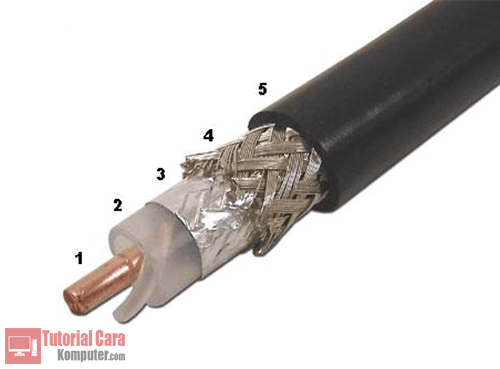
\includegraphics[width=1\textwidth]{figures/bgncoax.png}}
	\caption{Gambar Bagian - Bagian pada Kabel Coaxial}
	\label{bgncoax}
	\end{figure}
	Gambar \ref{bgncoax} ini adalah bagian bagian yang terdapat pada kabel coaxial. 
	
		\begin{enumerate}
			\item Pada bagian paling dalam kabel COaxial terdapat kabel tembaga yang dimana kabel tersebut berfungsi sebagai media pengantar aliran listrik.
			\item Lapisan plastik, lapisan ini fungsinya menjadi pemisah antara kabel tembaga dan lapisan metal yang membalutnya.
			\item Lapisan metal, lapisan ini sebagai pelindung bagian inti kabel, dan berfungsi pula sebagai pelindung dari pengaruh gelombang elektromagnetik dar luar kabel.
			\item Pelindung (Grounding), memiliki fungsi untuk membantu pita tembaga dalam mengurangi pengaruh gangguan frekuensi liar dan juga sebagai grounding.
			\item Lapisan plastik terluar, bagian yang melindungi keseluruhan bagian kabel yang berada di dalam kabel.
		\end{enumerate}
		
	Berikut ini beberapa kelebihan dan kekurangan pada kabel Coaxial :
		\begin{itemize}
 			\item Kelebihan
				\begin{enumerate}
					\item Kabel Coaxial relatif memiliki harga yang murah
					\item Kecepatan transmisi yg di miliki kabel Coaxial relatif tinggi, walupun memiliki batasan - batasan jangkauan tertentu
					\item Teknologi yang di terapkan pada jaringan kabel Coaxial masih terbilang sangat umum dan mudah untuk dipahami, dan yang lainnya.
				\end{enumerate}
				
			\item Kekurangan
				\begin{enumerate}
					\item Dalam urusan pemeliharaan dan perawatan biaya yang dikeluarkan relatif mahal.
					\item Mempunyai sifat yang rentan pada suhu dan temperatur.
					\item Jangkauan sinyal yang sangat terbatas, sehingga memerlukan sebuah repeater lagi untuk menambahkan sinyal jarak jauh, dan yang lainnya.
					\item untuk proses penginstallannya pun kabel coaxial ini termasuk rumit, dikarenakan butuh ketelitian dan kejelian untuk ukuran dari kabel coaxial tersebut
					\item jika kabel ini dipasang di bawah tanahpun rentan sekali terkena gangguan-gangguan fisik yang membuat terputusnya kabel ini, contohnya jika ada gempabumi atau ada tikus tanah dan sebagainya.
				\end{enumerate}
		\end{itemize}
		
\subsection {Karakteristik Kabel Coaxial}
	Kabel coaxial memiliki perlindungan intrefensi, dengan maksimal bandwithnya yaitu 10 mbps. Kabel coaxial mempunyai panjang maksimal 500 meter dengan soket atau konektor menggunakan jenis BNC (Bayonet Noval Conector). Harga kabel coaxial relatif lebih murah dibanding kabel fiber optik. Jenis topologi yang biasa diterapkan untuk kabel coaxial ada dua yaitu topologi BUS dan Topologi Ring. Dan untuk instalasi pemasangan kabel coaxial bisa dibilang cukup mudah dan terbilang sederhana.
	
\subsection{Tipe Kabel Coaxial}
		\subsubsection{Thick coaxial cable(Kabel koaksial ``Gemuk``)}
		kabel coaxial jenis ini dispesifikasikan berdasarkan standar IEEE 802.3 - 10BASE5, dimana kabel ini mempunyai diameter rata-rata 12mm. kabel ini biasa disebut sebagai standard ethernet atau thick ethernet(ThickNet), bahkan hanya disebut dengan yellow cabel karena warnanya yang kuning.
		kabel coaxial ini jika digunakan dalam jaringan mempunyai spesifikasi dan aturan sebagai berikut:
			\begin{enumerate}
				\item Setiap ujung harus diterminasi dengan terminator 50ohm(dianjurkan menggunakan terminator yang telah dirakit)
				\item Maksimum 3 Segment dengan peralatan terhubung (attached devices).
				\item Setiap kartu jaringan mempunyai pemancar tambahan.
				\item Setiap segment maksimum berisi 100 perangkat jaringan, termasuk dalam hal ini repeaters.
				\item maksimum panjang kabel per segment adalah 1.640 feet(sekitar 500meter).
				\item Maksimum jarak antar segment adalah 4.920 feet(sekitar 1500 meter).
				\item Setiap segment harus dieri ground.
				\item Jarak maksimum antara tap atau pancabanga dari kabel utama ke perangkat adalah 16 feet (sekitar 5 meter).
			\end{enumerate}
\begin{figure} [ht]
	\centerline{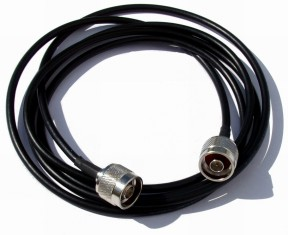
\includegraphics[width=1\textwidth]{figures/thickcoax.jpg}}
	\caption{Gambar Kabel Coaxial Thick}
	\label{thickcoax}
\end{figure}
	Gambar \ref {thickcoax} ini adalah sebuah gambaran tentang kabel coaxial thick.
	
		\subsubsection{Thin coaxial cable (kabel coaxial ``kurus``)}
		Kabel Coaxial jenis ini banyak dipergunakan di kalangan radio amatir, terutama untuk transciever yang tidak memerlukan output daya yang besar. Jenis yang banyak digunakan RG-8 atau RG-59 dengan impedansi 75 ohm. Jenis kabel untuk televisi juga termasuk jenis coaxial.
		Namun untuk perangkat jaringan, kabel jenis coaxial yang dipergunakan adalah (RG-58) yang telah memenuhi standar IEEE 802.3 - 10BASE2, dimana diameter rata-rata berkisar 5mm dan biasanya berwarna hitam. setiap perangkat (device) dihubungkan dengan BNC T-connector.
		Kabel coaxial jenis ini , misalnya jenis RG-58 A/U atau C/U, jika si-implementasikan dengan T-connector dan terminator dalam sebuah jaringan harus mengikuti standar berikut :
			\begin{enumerate}
				\item Setiap ujung kabel diberi terminator 50 ohm.
				\item Panjang maksimal kabel adalah 606.8 feet (185 meter) per segment.
				\item Setiap segment maksimum terkoneksi sebanyak 30 perangkat jaringan (devices)
				\item Kartu jaringan cukup tambagan transceiver yang onboard, tidak perlu tambahan transceiver, kecuali yang repeater.
				\item Maksimum ada 3 segment terhubung satu sama lain.
				\item Setiap segment sebaiknya dilengkapi 1 ground.
				Panjang minimum antar T-connector adalah 1,5 feet (0.5 meter).
				\item Maksimum panjang kabel dalam satu segment adalah 1.818 feet (555 meter).
				\item Setiap segment maksimum mempunyai 30 perangkat terkoneksi.
			\end{enumerate}
\begin{figure} [ht]
	\centerline{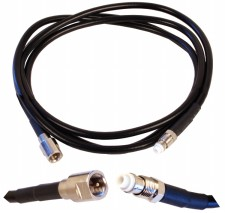
\includegraphics[width=1\textwidth]{figures/thincoax.jpg}}
	\caption{Gambar Kabel Coaxial Thin}
	\label{thickcoax}
\end{figure}
Gambar \ref{thincoax} adalah contoh gambar kabel coaxial thin.

\subsection{Sejarah Kabel Coaxial}
	Dari hasil kelanjutan penemuan bentuk saluran yang menggunakan dua kawat yang sudah pernah digunaka di periode sebelumnya, kabel Coaxial pun berkembang di tahun 1920. Di daerah perkotaan bagian Amerika Timur, kabel Coaxial hasil buatan Laboratorium Bell di gunakan untuk menghubungkan antar kota. Kabel Coaxial ternyata terbukti bisa di gunakan untuk menyalurkan isi informasi siaran, sewaktu teknologi televisi sedang populer. Laboratorium Bell terus mengembangkan peralatan multipeks dan repeater (penunjang) pada tahun - tahun berikutnya, agar sistem transmisi menjadi lebih efisien. Dengan harapan dapat mengurangi biaya konstruksi dan pemeliharaan, di akhir tahun 1960, kabel Coaxial di gunakan pada sistem mikrowave.
	
\subsection{Jenis Jenis Konektor Kabel Coaxial}
		\begin{enumerate}
			\item Konektor FC
			Jenis konektor ini menggunakan drat ulir yang posisinya dapat di atur, sehingga ketika dipasang, akurasinya tidak berubah, Jenis kabel single mode dengan akurasi yang tinggi sbg penghubung kabel dengan transmitter atau reciever.
			\item Konektor SC
			Jenis konektor ini bisa dicopot pasang. akurasinya dapat diatur manual dengan perangkat, sederhana dan relatif murah.
			\item Konektor ST
			Berbentuk seperti bayonet dan hampir mirip dengan konektor BNC.
			\item Konektor Biconic
			Konektor yang mucul pertama kali dalam komunikasi fiber optik dan sudah jarang digunakan.
			\item Konektor SMA
			Konektor yang menjadi pendahulunya dari konektor ST
			\item Konektor D4
			Konektor yang mirip seperti konektor FC, hanya saya ukuran yang berbeda.

		\end{enumerate}
	\subsection {Penerapan Kabel Coaxial Pada Jaringan Komputer}

	Dalam penerapannya, Instalasi pemasangan kabel coaxial harus dilakukan dengan sangat rapi dan hati-hati. Perhitungan kabel jaringan coaxial harus diukur dengan sangat sempurna karena jika salah dalam perhitungan ukuran dapat mengakibatkan rusaknya NIC (Network Interface Card) yang dipergunakan. Selain dapat merusak NIC, Kesalahan pengukuran kabel jaringan coaxial dalam instalasi pemasangan juga memberikan dampak pada kinerja jaringan itu sendiri yang akan terhambat karena jaringan tidak mencapai kemampuan maksimalnya.Ada beberapa hal yang perlu diperhatikan dalam instalasi pemasangan kabel coaxial untuk mendapatkan hasil yang sempurna:
		\begin{itemize}
			\item Kontinuitas konduktor utama kabel coaxial harus dalam kondisi baik dan terpelihara
			\item Pada sambungan kabel coaxial harus ketat sehingga kabel tersebut tetap bersifat homogen seperti pada kondisi awal
			\item Redaman yang didapatkan harus bisa tetap pada angka nol atau sekecil-kecilnya
			\item Hasil dari pekerjaan sambungan kabel coaxial tersebut harus benar-benar rapi.
		\end{itemize}
		
	Kabel Coaxial biasa digunakan untuk mentransmisikan sinyal frekuensi tinggi mulai dari 300 kHz ke atas. Di karenakan memiliki kemampuan untuk menyalurkan frekuensi tinggi, maka sistem transmisi menggunakan kabel Coaxial mempunyai kapasitas kanal yang cukup besar.
	
\begin{figure} [ht]
	\centerline{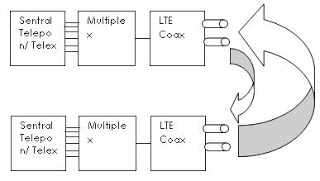
\includegraphics[width=1\textwidth]{figures/multiplex.JPG}}
	\caption{Gambar Multiplex}
	\label{multiplex}
\end{figure}	
	\ref{multiplex}
	Pada gambar di atas ini yang di maksudkan adalah alat yang di gunakan untuk menyusun kanal telepon menjadi suatu band frekuensi terntentu (base band) atau pun sebaliknya, Sedangkan LTE (Line Terminal Equipment) Coaxial ialah interface antara multiplex dengan kabel Coaxial.

